\begin{frame}{List, dict, set comprehension}
    \lstinputlisting{introduction/code/addons/comprehension.py}
\end{frame}

\begin{frame}{Płaski model pamięci}
    \begin{table}
        \centering
        \begin{tabular}{rc|c|}
            \cline{3-3}
            & & \\
            \cline{3-3}
            0x8000 & $\longrightarrow$ & $\cdots$ \\
            \cline{3-3}
            0x8001 & $\longrightarrow$ & 01110010 \\
            \cline{3-3}
            0x8002 & $\longrightarrow$ & 10010101 \\
            \cline{3-3}
            0x8003 & $\longrightarrow$ & 11011011 \\
            \cline{3-3}
            0x8004 & $\longrightarrow$ & 10111011 \\
            \cline{3-3}
            0x8005 & $\longrightarrow$ & 11110010 \\
            \cline{3-3}
            0x8006 & $\longrightarrow$ & 01110001 \\
            \cline{3-3}
            0x8007 & $\longrightarrow$ & 10110011 \\
            \cline{3-3}
            0x8008 & $\longrightarrow$ & 00101100 \\
            \cline{3-3}
            0x8009 & $\longrightarrow$ & $\cdots$ \\
            \cline{3-3}
            & & \\
            \cline{3-3}
        \end{tabular}
    \end{table}
\end{frame}

\begin{frame}{Przypisanie w pamięci}
    \begin{columns}
        \begin{column}{0.4\textwidth}
            \lstinputlisting{introduction/code/addons/memory_assignment_1.py}
            \begin{table}
                \centering
                \begin{tabular}{rc|c|}
                    \cline{3-3}
                    a & $\longrightarrow$ & 1 \\
                    \cline{3-3}
                    \\
                    \cline{3-3}
                    ? & $\longrightarrow$ & 1 \\
                    \cline{3-3}
                    a & $\longrightarrow$ & 2 \\
                    \cline{3-3}
                \end{tabular}
            \end{table}
        \end{column}
        \begin{column}{0.4\textwidth}
            \lstinputlisting{introduction/code/addons/memory_assignment_2.py}
            \begin{table}
                \centering
                \begin{tabular}{rc|c|}
                    \cline{3-3}
                    a & $\longrightarrow$ & 1 \\
                    \cline{3-3}
                    b & \multicolumn{1}{c}{$\nearrow$} & \multicolumn{1}{c}{} \\
                    \\
                    \cline{3-3}
                    a & $\longrightarrow$ & 2 \\
                    \cline{3-3}
                \end{tabular}
            \end{table}
        \end{column}
    \end{columns}
\end{frame}

\begin{frame}{Listy w pamięci}
    W wielu miejscach w pythonie korzystamy z referencji (wskaźników). W liście nie trzymamy wartości zmiennych, a wskaźniki na miejsca w których wartości zmiennych się znajdują. Dlatego mnożąc listę, mnożymy wskaźniki, a nie wartości. Następnie zmieniamy wartość na którą wskazuje wskaźnik, a nie sam wskaźnik.
    \lstinputlisting{introduction/code/addons/memory_assignment_3.py}
\end{frame}

\begin{frame}{Zmienne zmienne i niezmienne}
    Wartości zmiennych (variable) mogą być zmienne, mutowalne (mutable) lub niezmienne, niemutowalne (immutable). \\
    Wartości mutowalne mogą zmieniać swoją wartość w trakcie trwania programu. \\
    Wartości niemutowalne nie mogą się zmieniać - trzeba stworzyć nową wartość zmieniając część z jej części składowych. \\
    \lstinputlisting{introduction/code/addons/mutable.py}
\end{frame}

\begin{frame}{Ułamki}
    \begin{justify}
        Zauważmy, że:
        \begin{itemize}
            \item Każdy ułamek dziesiętny skończony lub nieskończony okresowy można zamienić w ułamek zwykły.
            Jedynie ułamka dziesiętnego nieskończonego nieokresowego nie da się zamienić. \\
            \item Każdy ułamek zwykły nieskracalny o mianowniku, będącym dzielnikiem
            jakiejś potęgi liczby 10 da się zamienić w ułamek dziesiętny skończony. \\
            \item Każdy ułamek zwykły nieskracalny o mianowniku niemającym tej własności
            jest równy pewnemu ułamkowi dziesiętnemu nieskończonemu okresowemu. \\
        \end{itemize}

        Ponieważ każdy ułamek zwykły to iloraz dwóch liczb całkowitych, więc każdy ułamek dziesiętny
        skończony lub nieskończony okresowy da się zapisać w postaci dwóch liczb całkowitych.
    \end{justify}
\end{frame}
\begin{frame}{Przeliczanie ułamków okresowych na zwykłe}
    \begin{gather*}
        0,(1234) = x | * 10000 \\
        1234,(1234) = 10000x \\
        1234,(1234) = 1234 + x \\
        1234 = 9999x \\
        x = \frac{1234}{9999} \\
        0,(1234) = \frac{1234}{9999} \\
    \end{gather*}
\end{frame}

\begin{frame}{Liczby rzeczywiste}
    Każda liczba rzeczywista jest jakimś ułamkiem dziesiętnym(również nieskończonym nieokresowym).

    Komputer jest maszyną skończoną i jako taki ma ograniczone zasoby. Z tego powodu w komputerze
    nie może przechowywać dokładnie niektórych rodzajów danych. Przykładem są liczby rzeczywiste,
    których jest nieskończenie wiele i których większość posiada nieskończone rozwinięcia dziesiętne.

    Rozpatrzmy liczbę $\pi$, która pozwoli nam lepiej zrozumieć problem.
    Poniżej przedstawiam jedynie pierwszych 1500 cyfr po przecinku jej rozwinięcia dziesiętnego.

\end{frame}
\begin{frame}{Pi, czyli 3,\dots}
    \centering
    14159265358979323846264338327950288419716939937510
    58209749445923078164062862089986280348253421170679
    82148086513282306647093844609550582231725359408128
    48111745028410270193852110555964462294895493038196
    44288109756659334461284756482337867831652712019091
    45648566923460348610454326648213393607260249141273
    72458700660631558817488152092096282925409171536436
    78925903600113305305488204665213841469519415116094
    33057270365759591953092186117381932611793105118548
    07446237996274956735188575272489122793818301194912
    98336733624406566430860213949463952247371907021798
    60943702770539217176293176752384674818467669405132
    00056812714526356082778577134275778960917363717872
    14684409012249534301465495853710507922796892589235
    42019956112129021960864034418159813629774771309960
\end{frame}
\begin{frame}{Pi, a dalej \dots}
    \centering
    51870721134999999837297804995105973173281609631859
    50244594553469083026425223082533446850352619311881
    71010003137838752886587533208381420617177669147303
    59825349042875546873115956286388235378759375195778
    18577805321712268066130019278766111959092164201989
    38095257201065485863278865936153381827968230301952
    03530185296899577362259941389124972177528347913151
    55748572424541506959508295331168617278558890750983
    81754637464939319255060400927701671139009848824012
    85836160356370766010471018194295559619894676783744
    94482553797747268471040475346462080466842590694912
    93313677028989152104752162056966024058038150193511
    25338243003558764024749647326391419927260426992279
    67823547816360093417216412199245863150302861829745
    55706749838505494588586926995690927210797509302955
\end{frame}
\begin{frame}{Liczby zmiennoprzecinkowe}
    Automat skończony jakim jest komputer nie mamy możliwości reprezentowania wszystkich liczb
    rzeczywistych, a jedynie ich mniej lub bardziej dokładne przybliżenia - mówi się, że float
    reprezentuje liczby zmiennoprzecinkowe, ponieważ w pamięci trzymane są w postaci znormalizowanej
    (czyli z przesuniętym przecinkiem) jako mantysa i wykładnik\footnote{zgodnie ze standardem IEEE 754}.
    \begin{center}
        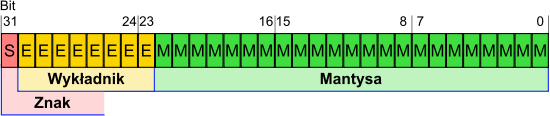
\includegraphics[width=0.7\textwidth]{introduction/graphics/ieee_full.png}
    \end{center}
\end{frame}

\begin{frame}{Przeliczanie liczb zmiennoprzecinkowych}
    \begin{center}
        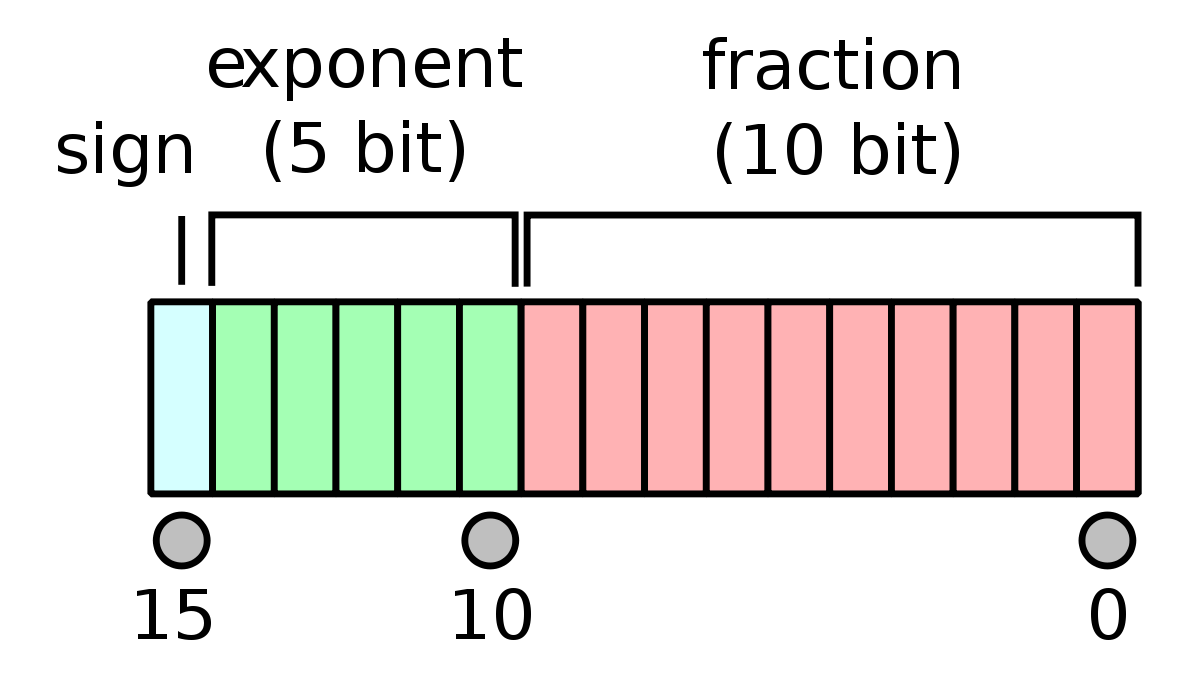
\includegraphics[height=0.2\textheight]{introduction/graphics/ieee_half.png} \\
        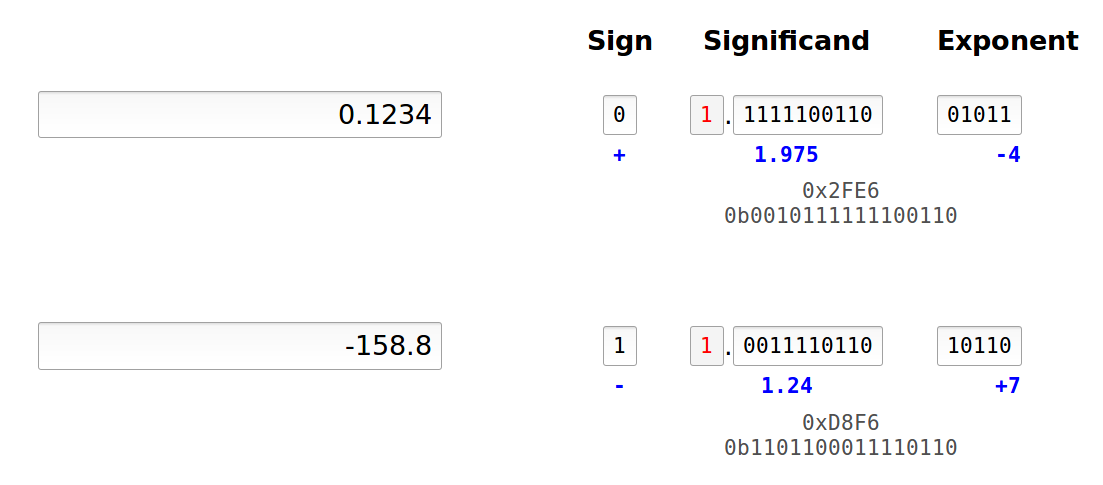
\includegraphics[height=0.45\textheight]{introduction/graphics/calculations.png}
    \end{center}
    Program do przeliczania dla różnych precyzji: \url{http://weitz.de/ieee/}
\end{frame}

\begin{frame}{Problem dużej tablicy}
    Przyjmijmy, że jesteśmy twórcą książki telefonicznej dla miasteczka, którego mieszkańcy mają
    dziwne, 10 literowe nazwiska. Aby zapewnić, że dla każdego możliwego nazwiska znajdzie się
    miejsce w naszej tablicy, musielibyśmy zapewnić jej rozmiar co najmniej 26^{10}. \\
    Jeśli w mieście żyje kilkanaście osób, zmarnujemy bardzo dużo pamięci. \\
    Na potrzeby rozwiązania skorzystajmy z 10 elementowej tablicy i funkcji skrótu znanej z numerologii.
    Zupełnie nie przejmujmy się tym, że ta funkcja ma beznadziejne własności.
    \begin{table}
        \centering
        \begin{tabular}{|c|c|c|c|c|c|c|c|c|}
            \hline
            1 & 2 & 3 & 4 & 5 & 6 & 7 & 8 & 9 \\
            \hline
            A & B & C & D & E & F & G & H & I \\
            J & K & L & M & N & O & P & Q & R \\
            S & T & U & V & W & X & Y & Z & \\
            \hline
        \end{tabular}
    \end{table}
\end{frame}
\begin{frame}{Obliczanie funkcji skrótu}
    Wartość numeryczna nazwiska KABARETKID wynosi 2121952294 $\rightarrow$ 37 $\rightarrow$ 10 $\rightarrow$ 1. \\
    MATEMATYKA $\rightarrow$ 4125412721 $\rightarrow$ 29 $\rightarrow$ 11 $\rightarrow$ 2 \\
    DELFINADDA $\rightarrow$ 4536951441 $\rightarrow$ 42 $\rightarrow$ 6 \\
    COPERNICON $\rightarrow$ 3675959365 $\rightarrow$ 58 $\rightarrow$ 13 $\rightarrow$ 4 \\
    MOCZYMORDA $\rightarrow$ 4638746941 $\rightarrow$ 52 $\rightarrow$ 7 \\
    WIBRAKACJA $\rightarrow$ 5929121311 $\rightarrow$ 34 $\rightarrow$ 7 \\
    Wartości trafiają pod odpowiednie pola tablicy, a w przypadku wystąpienia konfliktu...
    Jednym z rozwiązań jest trzymanie w tablicy wielu małych list, do których dodajemy wartości
    z kluczem o tej samej skróconej wartości. \\
    Dobra funkcja skrótu rozrzuca wartości równomiernie po całej tablicy, chociaż konflikty zawsze
    będą się zdarzały - co jest nieuniknione, gdy liczba elementów przekroczy rozmiar tablicy.
\end{frame}
\begin{frame}{Binarne drzewo poszukiwań -BST}
    \begin{center}
        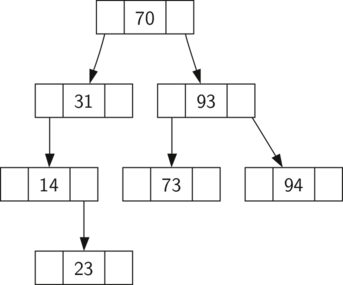
\includegraphics[height=0.8\textheight]{introduction/graphics/bst.png}
    \end{center}
\end{frame}

\begin{frame}{Notacja polska, Odwrotna notacja polska}
    Notacja polska (NP) - zapis przedrostkowy, notacja Łukasiewicza, zapis prefiksowy (prefix - przedrostek), normal Polish notation (NPN) \\
    Odwrotna notacja polska (ONP) - zapis przyrostkowy, notacja Azciweisakuł, zapis postfiksowy (postfix, sufix - przyrostek), reverse Polish notation (RPN) \\
    \begin{columns}
        \begin{column}{0.5\textwidth}
            NP:
            \[ +_1 +_2 0_1 0_2 0_3 = \]
            \[ ( 0_1 +_2 0_2 ) +_1 0_3 \]
            \[ +_1 0_1 +_2 0_2 0_3 = \]
            \[ 0_1 +_1 ( 0_2 +_2 0_3 ) \]
        \end{column}
        \begin{column}{0.5\textwidth}
            ONP:
            \[ 0_3 0_2 0_1 +_2 +_1 = \]
            \[ 0_3 +_1 ( 0_2 +_2 0_1 ) \]
            \[ 0_3 0_2 +_2 0_1 +_1 = \]
            \[ ( 0_3 +_2 0_2 ) +_1 0_1 \]
        \end{column}
    \end{columns}
    Zauważ, które działania są swoimi odbiciami lustrzanymi, a które odbiciami znaczeniowymi.
\end{frame}

\begin{frame}{Prefix, infix, postfix}
    \begin{columns}
        \begin{column}{0.3\textwidth}
            Notacja prefixowa:
            \[ +_1 0_1 0_2 = \]
            \[ +_1 +_2 0_1 0_2 0_3 = \]
            \[ +_1 0_1 +_2 0_2 0_3 = \]
            \[ +_1 +_2 +_3 0_1 0_2 0_3 0_4 = \]
            \[ +_1 +_2 0_1 +_3 0_2 0_3 0_4 = \]
            \[ +_1 +_2 0_1 0_2 +_3 0_3 0_4 = \]
            \[ +_1 0_1 +_2 +_3 0_2 0_3 0_4 = \]
            \[ +_1 0_1 +_2 0_2 +_3 0_3 0_4 = \]
        \end{column}
        \begin{column}{0.4\textwidth}
            Notacja infixowa:
            \[ 0_1 +_1 0_2 = \]
            \[ ( 0_1 +_2 0_2 ) +_1 0_3 = \]
            \[ 0_1 +_1 ( 0_2 +_2 0_3 ) = \]
            \[ ( ( 0_1 +_3 0_2 ) +_2 0_3 ) +_1 0_4 = \]
            \[ ( 0_1 +_2 ( 0_2 +_3 0_3 ) ) +_1 0_4 = \]
            \[ ( 0_1 +_2 0_2 ) +_1 ( 0_3 +_3 0_4 ) = \]
            \[ 0_1 +_1 ( ( 0_2 +_3 0_3 ) +_2 0_4 ) = \]
            \[ 0_1 +_1 ( 0_2 +_2 ( 0_3 +_3 0_4 ) ) = \]
        \end{column}
        \begin{column}{0.3\textwidth}
            Notacja postfixowa:
            \[ 0_1 0_2 +_1 = \]
            \[ 0_1 0_2 +_2 0_3 +_1 = \]
            \[ 0_1 0_2 0_3 +_2 +_1 = \]
            \[ 0_1 0_2 +_3 0_3 +_2 0_4 +_1 = \]
            \[ 0_1 0_2 0_3 +_3 +_2 0_4 +_1 = \]
            \[ 0_1 0_2 +_2 0_3 0_4 +_3 +_1 = \]
            \[ 0_1 0_2 0_3 +_3 0_4 +_2 +_1 = \]
            \[ 0_1 0_2 0_3 0_4 +_3 +_2 +_1 = \]
        \end{column}
    \end{columns}
\end{frame}

\begin{frame}{Bramki logiczne wg ANSI}
    \begin{table}
        \centering
        \begin{tabular}{|c|c|c|c|}
            \hline
            NOT & AND & OR & XOR \\
            \hline
            $\lnot$, $\sim$ & $\land$ & $\lor$ & $\veebar$ \\
            \hline
            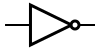
\includegraphics[width=0.25\textheight]{src/introduction/graphics/gates/NOT_ANSI.png} & 
            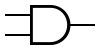
\includegraphics[width=0.25\textheight]{src/introduction/graphics/gates/AND_ANSI.png} &
            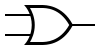
\includegraphics[width=0.25\textheight]{src/introduction/graphics/gates/OR_ANSI.png} &
            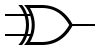
\includegraphics[width=0.25\textheight]{src/introduction/graphics/gates/XOR_ANSI.png} \\
            \hline
            \hline
            IMPLY & NAND & NOR & XNOR \\
            \hline
            $\implies$ & $\barwedge$ & $\barvee$ & $\iff$ \\
            \hline
            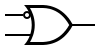
\includegraphics[width=0.25\textheight]{src/introduction/graphics/gates/IMPLY_ANSI.png} & 
            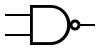
\includegraphics[width=0.25\textheight]{src/introduction/graphics/gates/NAND_ANSI.png} &
            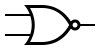
\includegraphics[width=0.25\textheight]{src/introduction/graphics/gates/NOR_ANSI.png} &
            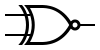
\includegraphics[width=0.25\textheight]{src/introduction/graphics/gates/XNOR_ANSI.png} \\
            \hline
        \end{tabular}
    \end{table}
\end{frame}
